\section{Simulation Experiments}
The evaluation separates the mechanical value of cable coupling from numerical planning performance. A parameterized strip family tests reachability; nine square warehouse tasks compare algorithms. Matched ablations, footprint variations, and a serial formation examine the contributing mechanisms and extensions.

\subsection{Unified Settings and Constructively Feasible Maps}
The implementation uses MATLAB R2024a, AMPL, Ipopt 3.12.13, BONMIN 1.8.9, and HSL MA57 on a Windows workstation with an Intel Core i9-12900 processor. MATLAB uses one computation thread, and optimization jobs run sequentially. All state updates and replay checks use first-order explicit Euler. Table~\ref{tab:settings} specifies the common geometry, tolerances, and computational settings.

\begin{table}[!t]
\centering\caption{Shared geometry, numerical settings, and validation thresholds}
\label{tab:settings}\footnotesize
\setlength{\tabcolsep}{4pt}
\begin{tabular}{ll}
\toprule
Quantity & Value\\
\midrule
Workspace & $16\times16$ m\\
Tractor footprint; wheelbase & $0.60\times0.70$ m; $0.40$ m\\
Nominal cart footprint & $1.05\times1.10$ m\\
Hitch-to-axle / rear overhang & $0.70/0.35$ m\\
Material cable length & $1.335$ m\\
Minimum turning radius & $0.40$ m\\
Endpoint lower bound / step bound & $0.25/0.18$ m\\
Heading bounds & $[-\pi,\pi]$ rad\\
Required / planning clearance & $0.10/0.12$ m\\
Curvature regularization $\gamma$ & $0.002$\\
Original-grid cart position bound & $0.12$ m per coordinate\\
Original-grid cart heading bound & $0.008$ rad\\
Tractor terminal heading bound & $10^{-5}$ rad\\
Finer Euler replay subdivisions & $8$ per interval\\
Fine cart position / heading bounds & $0.27$ m per coordinate / $0.025$ rad\\
Common computation allowance & $30$ s\\
Direct NLP iteration ceiling & $3000$\\
Relaxed stage allowance / iterations & $5$ s / $300$\\
Relaxation product bound & $10^{-4}$ m$^2$\\
Refinement iteration ceiling & $600$\\
Initial restoration / final reserve & $4/4$ s\\
Initial restoration weights & $1/8,1/32,1/128,1/512,1/1024$\\
Final recovery weights & $1,1/2,\ldots,1/1024$\\
Yaw projection bisections & $65$\\
Terminal correction iterations & At most $5$\\
Terminal correction window & $\min\{N,\max\{9,\lceil N/4\rceil\}\}$\\
PORT unique schedules / allowance & At most $3$ / $30$ s\\
\bottomrule
\end{tabular}
\end{table}

The tractor polygon is referenced to its rear axle and extends forward. The cart polygon extends to either side of its axle; its front hitch lies at the forward center. The cable joins the tractor rear axle to that hitch, as defined in Fig.~\ref{fig:kinematics}. Complete vertices, maps, controls, source code, solver inputs, logs, and validation records are available in the reproducibility package at \url{https://anonymous.4open.science/r/Cable-Towing-Trailer-361F/}. Its README maps each comparison to the source files and records, with file hashes for integrity checks.

The nine layouts are defined by modular rack rows, picking aisles, cross aisles, pallet staging areas, and packing stations before trajectory construction. Their common outer boundary is $16\times16$ m. W01--W09 respectively represent a blocked-aisle transfer, a two-aisle rack-end transfer, a cross-aisle exchange, an adjacent-aisle return, two successive offsets between storage blocks, a packing-area turn, a pallet-staging bypass, a return between mixed rack orientations, and a perimeter replenishment circuit. The nominal picking aisles in W01--W08 are $1.7$ m wide for a $1.1$ m cart; cross aisles provide the space needed for the complete formation to turn. Discrete racks leave connected access routes and functional work areas.

Feasible control sequences are constructed within the fixed layouts and checked by the common validator. All comparisons use the same nine maps, accepted seeds, model parameters, and physical acceptance criteria. A single configuration of the proposed method is applied across this designed benchmark.

\begin{table}[!t]
\centering\caption{Warehouse layouts, meshes, and minimum replayed body clearances}
\label{tab:cases}
\footnotesize\begin{tabular}{lrrrr}
\toprule
Case & $N$ & Objects & Seed (m) & Proposed (m)\\
\midrule
W01 & 98 & 11 & 0.126 & 0.113\\
W02 & 135 & 8 & 0.196 & 0.168\\
W03 & 100 & 11 & 0.137 & 0.126\\
W04 & 142 & 12 & 0.170 & 0.159\\
W05 & 100 & 12 & 0.103 & 0.122\\
W06 & 91 & 12 & 0.162 & 0.119\\
W07 & 106 & 11 & 0.111 & 0.127\\
W08 & 127 & 12 & 0.197 & 0.182\\
W09 & 300 & 12 & 0.142 & 0.207\\
\bottomrule\end{tabular}
\end{table}

Table~\ref{tab:cases} reports the map obstacles, mesh sizes, and minimum body clearances under finer replay for the common initial trajectories and final proposed outputs. Figure~\ref{fig:nine-cases} uses identical physical map dimensions, canvas sizes, and vehicle scale. Cyan and green denote the tractor and cart; orange racks, yellow pallets, and violet packing stations identify distinct warehouse objects. Faint footprints show swept body positions. S and G mark the starting and final tractor configurations. Statistics include all nine layouts.

\begin{figure*}[!t]
\centering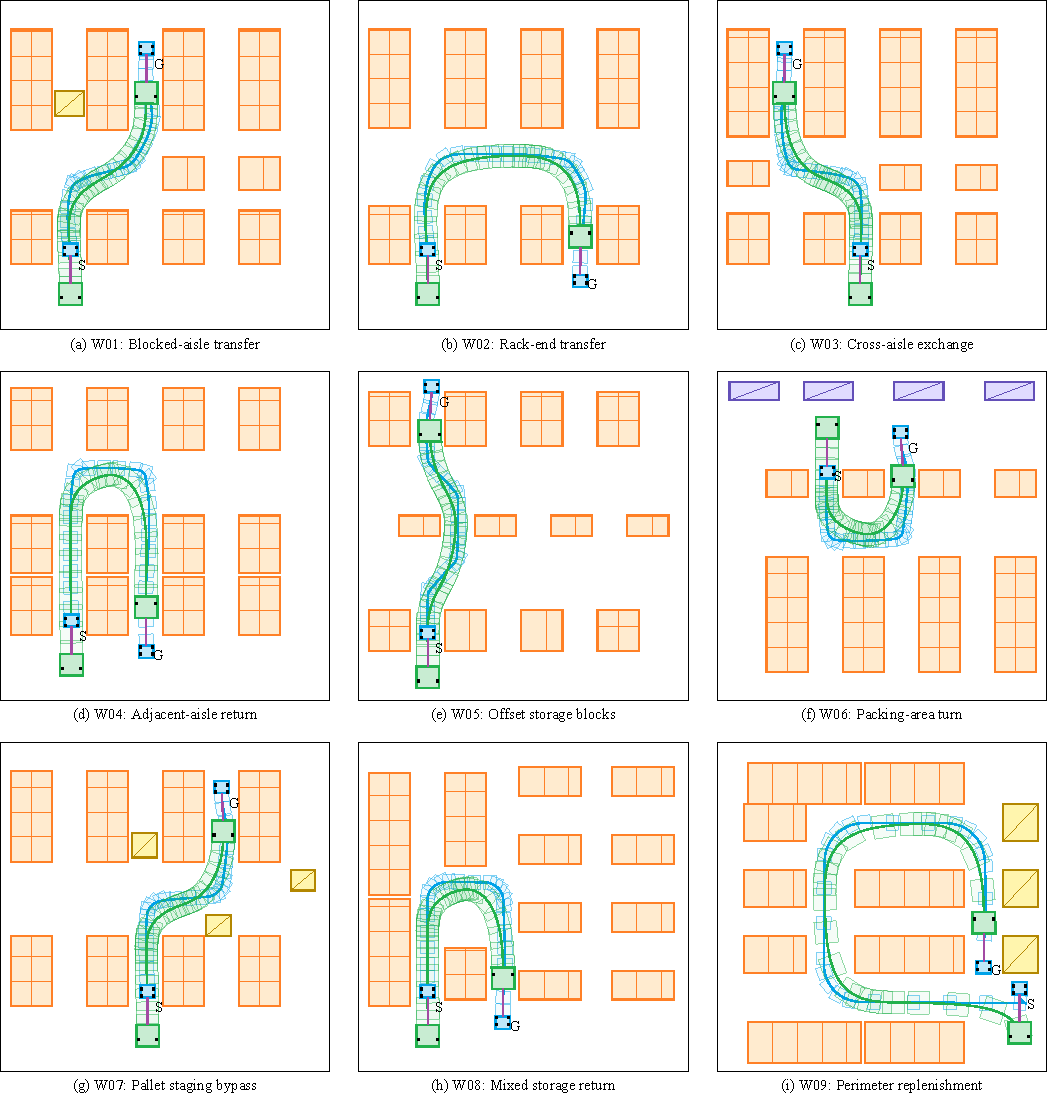
\includegraphics[width=\textwidth]{warehouse_cases.pdf}
\caption{Nine distinct confined warehouse tasks with identical workspace dimensions and vehicle scale.}
\label{fig:nine-cases}
\end{figure*}

All cable strategies receive the same feasible control seed, mesh, goal, physical clearance, and dual initialization for each map. Method order rotates across cases. The study measures trajectory improvement from constructive feasible initializations. The nominal allowance allocates optimization-stage time; reported elapsed time also includes pipeline overhead. Measured backend time includes serialization, startup, validation, and termination overhead. Time-limited outputs can be accepted if they pass all independent checks.

The transport tasks terminate in arrival regions around the prescribed cart pose. Both endpoint tests use that same goal: original-grid position and heading bounds are $0.12$ m per coordinate and $0.008$ rad; finer Euler replay uses $0.27$ m and $0.025$ rad. Across the nine proposed outputs, the actual finer-replay Euclidean position errors range from $0.050$ to $0.155$ m, and the maximum cart heading error is $0.02197$ rad ($1.26^\circ$). The maximum original-grid Euclidean error is $0.1375$ m. Per-case errors are supplied with the numerical records. Required body clearance remains $0.10$ m at both resolutions. These endpoint conditions define warehouse transfer arrival; precision docking and tracking are subsequent control tasks.

\subsection{Mechanical Benefit Relative to a Rigid Drawbar}
The strip study varies cable length over $1.3$, $1.5$, and $1.7$ m, tractor turning radius over $0.4$ and $0.5$ m, and excess strip width over $0.30$, $0.60$, and $0.85$ times the barrier in~\eqref{eq:barrier}. The resulting 18 tasks satisfy Theorem~\ref{thm:rigid}. The rigid comparator uses the same body dimensions, fully extended initial span, clearance, and target heading, and may reverse. Its reorientation is excluded by the geometric barrier.

All 18 cable trajectories pass independent Euler replay and fixed-material-length cable-route checks. Figure~\ref{fig:mechanism} shows the mechanism: the tractor reverses and rotates while the cart waits, then resumes pulling. Endpoint separation decreases during repositioning without changing material length. Three compact cases require the asymmetric cable-route family, using shape parameters $\beta\in\{0,\pm0.25,\pm0.50,\pm0.75\}$ and a material-length residual below $10^{-7}$ m. The original-grid and finer-replay node configurations are checked; the vehicle trajectories are unchanged.

\begin{figure*}[!t]
\centering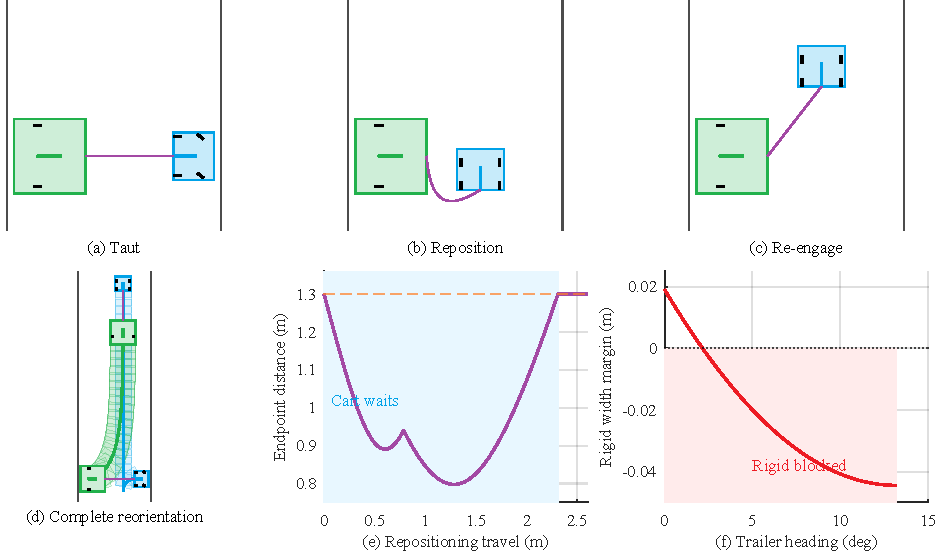
\includegraphics[width=\textwidth]{mechanism_revision.pdf}
\caption{Slack-enabled reorientation and the geometric obstruction imposed by an equal-length rigid drawbar.}
\label{fig:mechanism}
\end{figure*}

On the nine warehouse layouts, direct transcription with the rigid drawbar returns 0/9 new validated trajectories under the common allowance, compared with 8/9 for cable MAX. Both use the same footprints, taut connection length, task configurations, mesh, and direct nonlinear-solve strategy. Their shared initial controls are replayed through their respective kinematics; the resulting rigid rollout need not be feasible. The rigid cart may reverse. These attempts report numerical outcomes from that initialization, whereas Theorem~\ref{thm:rigid} independently establishes mechanical impossibility for the strip family. The controlled cable-algorithm comparison uses feasible initial trajectories for every method.


\subsection{Controlled Numerical Comparisons}
The comparisons evaluate feasible-seed trajectory refinement under the common discrete model. MAX, LOGIC, COMP, and MINLP compare representations of the same discrete cable relation. FIX and PORT compare mode strategies adapted from~\cite{zhang2026,yang2022}. After duplicate removal, PORT has one schedule on W01--W08 and three on W09; its single-schedule cases reduce to FIX, with separate time-limited runs. RGR uses replay reserves after causal rollout; the proposed method first restores a feasible initializer and includes final control recovery. Retained costs are recomputed from accepted controls. Mean travel reduction averages each case's reduction relative to its own common seed.

\begin{table*}[!t]
\centering\caption{Common-allowance comparison on nine warehouse tasks}
\label{tab:main}
\footnotesize\begin{tabular}{lrrrrrrr}
\toprule
Method & New & NLP & $\Delta J\geq1\%$ & $\Delta J$ (\%) & $\Delta l$ (\%) & $t_{50}$ (s) & $t_{90}$ (s)\\
\midrule
Proposed & 9/9 & 7/9 & 9/9 & 4.44 & 4.36 & 31.03 & 31.76\\
MAX & 8/9 & 8/9 & 6/9 & 1.02 & 0.97 & 30.97 & 33.91\\
LOGIC & 2/9 & 2/9 & 2/9 & 1.09 & 1.07 & 30.72 & 35.10\\
COMP & 2/9 & 2/9 & 2/9 & 0.91 & 0.91 & 30.68 & 32.32\\
FIX & 2/9 & 2/9 & 2/9 & 0.71 & 0.70 & 30.73 & 32.26\\
PORT & 3/9 & 3/9 & 2/9 & 0.78 & 0.77 & 31.12 & 34.03\\
MINLP & 0/9 & 0/9 & 0/9 & 0.00 & 0.00 & 31.41 & 32.10\\
RGR & 7/9 & 7/9 & 5/9 & 3.04 & 2.92 & 33.01 & 36.53\\
\bottomrule\end{tabular}
\end{table*}

Table~\ref{tab:main} distinguishes new validated planner outputs (New) from validated nonlinear-solver outputs before recovery (NLP); both counts have denominator nine. Every method retains a validated trajectory because the common feasible seed remains available. The proposed method produces 9/9 new outputs, including 7/9 accepted directly from its nonlinear solves, and improves the objective in all nine tasks. Its mean per-case travel reduction is 4.36\%, compared with 0.97\% for MAX; median backend times are 31.03 and 30.97 s. Its retained objective is lower than MAX in eight cases and lowest among the eight methods in four. MAX gives the lower objective on W09. The proposed method is faster than MAX in six cases, with comparable median time overall.
The objective reduction reaches at least one percent in 9/9 cases for Proposed and 6/9 for MAX. The statistics $t_{50}$ and $t_{90}$ denote median and 90th-percentile backend times. Together, these results support a quality and new-output acceptance advantage within the common computational allowance.


\begin{figure*}[!t]
\centering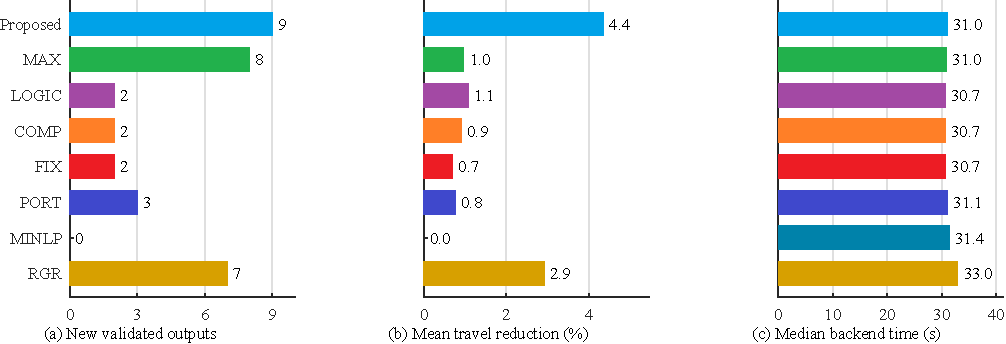
\includegraphics[width=.98\textwidth]{comparison_summary.pdf}
\caption{New validated trajectories, mean travel reduction, and measured backend time across all nine tasks.}
\label{fig:comparison}
\end{figure*}

\begin{table*}[!t]
\centering\caption{Retained objectives; asterisks mark no improvement over the common seed}
\label{tab:per-case}
\footnotesize\begin{tabular}{lrrrrrrrr}
\toprule
Case & Proposed & MAX & LOGIC & COMP & FIX & PORT & MINLP & RGR\\
\midrule
W01 & 12.12 & 13.15 & 13.29$^*$ & 13.29$^*$ & 13.29$^*$ & 13.29$^*$ & 13.29$^*$ & 12.83\\
W02 & 16.99 & 18.80 & 17.66 & 19.01$^*$ & 18.31 & 18.31 & 19.01$^*$ & 19.01$^*$\\
W03 & 12.47 & 13.09 & 13.23$^*$ & 13.23$^*$ & 13.23$^*$ & 13.23$^*$ & 13.23$^*$ & 12.13\\
W04 & 19.41 & 20.13 & 19.66 & 20.21$^*$ & 19.66 & 19.66 & 20.21$^*$ & 20.17\\
W05 & 13.09 & 13.13 & 13.33$^*$ & 13.33$^*$ & 13.33$^*$ & 13.33$^*$ & 13.33$^*$ & 12.78\\
W06 & 11.86 & 12.28$^*$ & 12.28$^*$ & 12.28$^*$ & 12.28$^*$ & 12.28$^*$ & 12.28$^*$ & 12.28$^*$\\
W07 & 12.80 & 12.98 & 13.07$^*$ & 13.07$^*$ & 13.07$^*$ & 13.07$^*$ & 13.07$^*$ & 12.25\\
W08 & 15.05 & 15.20 & 15.44$^*$ & 14.41 & 15.44$^*$ & 15.44$^*$ & 15.44$^*$ & 15.44$^*$\\
W09 & 31.23 & 30.98 & 31.60$^*$ & 31.11 & 31.60$^*$ & 31.41 & 31.60$^*$ & 30.01\\
\bottomrule\end{tabular}
\end{table*}

Figure~\ref{fig:details} compares the proposed and MAX tractor paths on the predeclared rack-end, double-offset, and perimeter tasks. Each panel includes the actual vehicle outlines and swept footprints. A route that shortens the tractor path is useful only if the passive cart and cable also satisfy validation. Figure~\ref{fig:modes} plots the perimeter task's initial repositioning phase against accumulated tractor travel. The transmitted cart displacement stays zero on slack steps while the tractor can move backward and change heading.

\begin{figure*}[!t]
\centering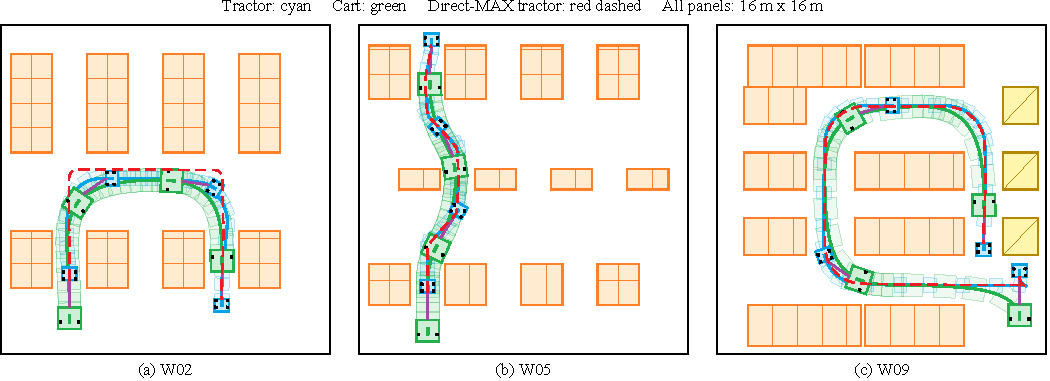
\includegraphics[width=.98\textwidth]{trajectory_details.pdf}
\caption{Validated paths and swept body footprints on three representative square warehouse tasks.}
\label{fig:details}
\end{figure*}

\subsection{Component Ablations and Repeated Runs}
The ablations test how individual stages contribute to accepted trajectory quality under fixed physical thresholds. Causal control restoration enforces consistency between controls and states, initial restoration supplies a validated refinement anchor, and replay reserves guide clearance during optimization. The paired recovery tests reuse identical preceding outputs, while the factorial study varies initial restoration and reserve treatment one factor at a time.

\begin{table*}[!t]
\centering\caption{Control-recovery ablations and solve-only strategy comparisons}
\label{tab:ablation}
\footnotesize\begin{tabular}{lrrrr}
\toprule
Variant & New & Impr. & $\Delta l$ (\%) & $t_{50}$ (s)\\
\midrule
Proposed & 9/9 & 9/9 & 4.36 & 31.03\\
No final recovery (paired) & 9/9 & 9/9 & 2.68 & 27.91\\
No terminal correction (paired) & 9/9 & 9/9 & 3.18 & --\\
RGR & 7/9 & 6/9 & 2.92 & 33.01\\
No reserves (RRP) & 0/9 & 0/9 & 0.00 & 31.78\\
MAX + recovery & 9/9 & 9/9 & 1.07 & 24.90\\
Relaxed stage only & 0/9 & 0/9 & 0.00 & --\\
\bottomrule\end{tabular}
\end{table*}

Both Proposed and MAX+recovery produce 9/9 new validated outputs. Their mean travel reductions are 4.36\% and 1.07\%, respectively, showing the quality benefit of the complete refinement workflow beyond adding recovery to MAX. Final recovery supplies four of the nine proposed outputs and raises mean reduction from 2.68\% at the identical paired prefix to 4.36\%. Removing terminal correction gives 3.18\%. The no-terminal-correction row reuses that same prefix, so a separate complete-pipeline runtime is inapplicable. The relaxed-only row reports first-stage acceptance and quality.

\begin{table*}[!t]
\centering\caption{Factorial comparison of initial restoration and three reserve settings}
\label{tab:factorial}
\footnotesize\begin{tabular}{lllrrrr}
\toprule
Variant & Initial restoration & Reserves & New & $\Delta J$ (\%) & $\Delta l$ (\%) & $t_{50}$ (s)\\
\midrule
F1 & On & Capped & 9/9 & 4.19 & 4.12 & 30.82\\
F2 & On & Uncapped & 9/9 & 4.58 & 4.49 & 30.77\\
F3 & On & Off & 9/9 & 3.41 & 3.35 & 31.03\\
F4 & Off & Capped & 8/9 & 2.82 & 2.75 & 30.74\\
F5 & Off & Uncapped & 9/9 & 2.93 & 2.85 & 31.12\\
F6 & Off & Off & 9/9 & 2.04 & 1.99 & 30.97\\
\bottomrule\end{tabular}
\end{table*}

Table~\ref{tab:factorial} crosses initial restoration with three reserve settings: zero, measured replay deviation, and deviation capped by available clearance. The cap retains half of the obstacle/wall surplus and divides half of the interbody surplus between the bodies. The overall allowance and physical acceptance rules remain fixed. With measured reserves, initial restoration increases mean travel reduction from 2.85\% (F5) to 4.49\% (F2). With restoration enabled, measured reserves give 4.49\%, compared with 3.35\% for zero reserves (F3) and 4.12\% for capped reserves (F1). F2 has the same configuration as Proposed and is a separate run within this matched experiment.
The capped variant F4 retains the common seed on W09 because the cap routine requires the stricter planning clearance at its initializer. Its seed still satisfies the shared physical acceptance threshold. The factorial results identify the quality contribution of restoration and measured reserves under these unchanged criteria.


The factorial table permits matched comparisons of initial restoration and reserve setting. The paired no-final-recovery result uses the exact outputs recorded before final recovery. The no-terminal-correction replay changes only that component and retains the original prefix. RGR--RRP removes only replay reserves from the solve-only workflow; MAX+recovery tests recovery on direct MAX. These comparisons identify the role of each design under unchanged physical acceptance rules.

\begin{figure*}[!t]
\centering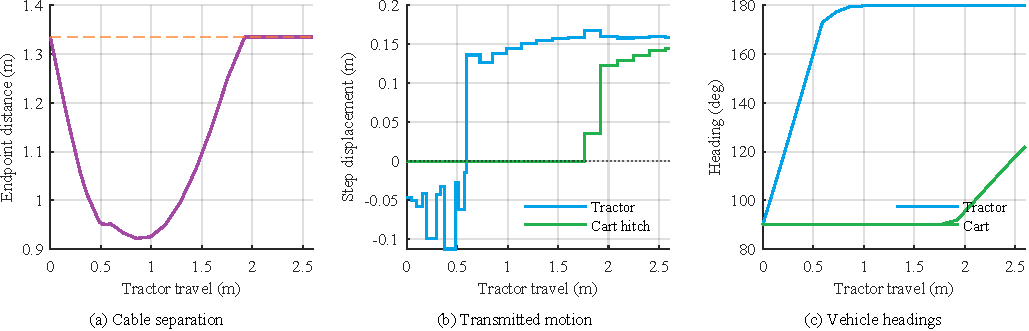
\includegraphics[width=\textwidth]{mode_evidence.pdf}
\caption{Cable distance, transmitted displacement, and vehicle headings during initial tractor repositioning.}
\label{fig:modes}
\end{figure*}

\begin{table*}[!t]
\centering\caption{Four-run sensitivity to numerical termination and process timing}
\label{tab:repeat}
\footnotesize\begin{tabular}{llrrrr}
\toprule
Case & Method & New & Objective range & $t_{50}$ (s) & IQR (s)\\
\midrule
W02 & Proposed & 4/4 & 16.99--17.00 & 30.77 & 0.18\\
W02 & MAX & 4/4 & 18.80--18.80 & 31.00 & 0.85\\
W05 & Proposed & 4/4 & 13.09--13.09 & 31.14 & 0.29\\
W05 & MAX & 4/4 & 13.13--13.13 & 30.71 & 0.02\\
W09 & Proposed & 4/4 & 31.17--31.24 & 32.99 & 0.63\\
W09 & MAX & 4/4 & 30.98--30.98 & 34.13 & 0.07\\
\bottomrule\end{tabular}
\end{table*}

Table~\ref{tab:repeat} includes the primary run and three additional runs on each fixed instance, measuring sensitivity to numerical termination and process timing. The task-dependent quality ordering persists: the proposed method has lower objectives on W02 and W05, while MAX has lower objectives on W09.

Repeated runs use the same three predeclared cases W02, W05, and W09, with three additional runs per method and case. They measure sensitivity to timing and numerical termination on fixed instances. An auxiliary LSE test changes only the mode expression of MAX at inverse scales $100$ and $1000$ m$^{-1}$ on those same cases. Its pointwise excess above a direct maximum is bounded by $\log 2/\rho$, where $\rho$ is the inverse scale, and it can transmit nonzero displacement while slack. Every smoothed output is checked against the exact cable relation.
The LSE variants return 0/3 and 0/3 outputs that pass the exact common validator at inverse scales 100 and 1000, respectively. They improve the common seed in 0/3 and 0/3 cases. These outcomes are evaluated under the exact cable relation rather than the smoothed surrogate. The final planner retains the direct maximum.


Figure~\ref{fig:budgets} varies the nominal allowance over 15, 30, and 60 s on W02, W05, and W09. It reports mean per-case travel reduction and newly validated outputs for Proposed, MAX, and MINLP. The horizontal coordinate of the quality plot is measured median backend time, including overhead; the acceptance plot uses the nominal allowance. All runs retain the same models, seeds, and acceptance rules. Longer allowances need not improve a nonconvex solve monotonically because they can change the intermediate candidates and time available for restoration.
At the 15-s allowance, Proposed and MAX produce 3/3 and 2/3 new validated outputs, with mean travel reductions of 4.27\% and 0.99\%. At the 60-s allowance, the corresponding median measured times are 38.95 and 61.20 s, and the mean travel reductions are 4.55\% and 1.45\%. These results describe the three fixed budget-test tasks.

\begin{figure*}[!t]
\centering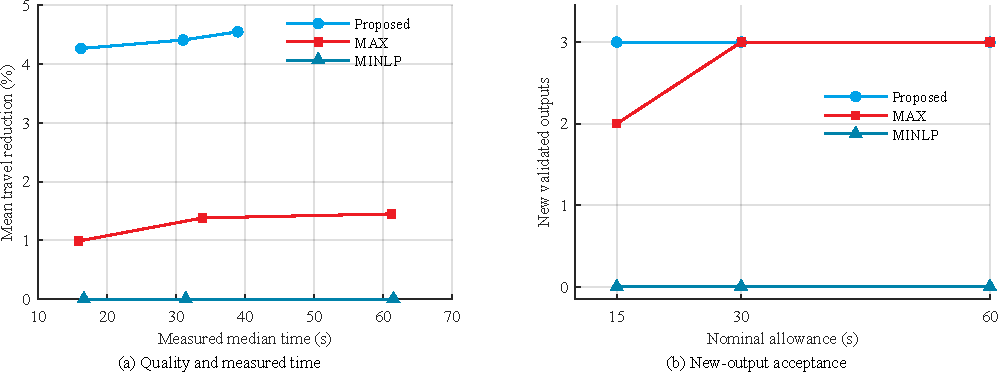
\includegraphics[width=\textwidth]{budget_sensitivity.pdf}
\caption{Quality and new-output acceptance under three nominal computation allowances on three fixed tasks.}
\label{fig:budgets}
\end{figure*}

\subsection{Footprint Variations and a Serial Formation}
Five cart geometries share the unchanged W02 warehouse, goal, cable length, kinematics, mesh, and initial controls. Only the cart polygon changes. S01--S05 respectively denote a nominal rectangle, compact rectangle, long narrow rectangle, irregular pentagon, and wide hexagon. Their actual vertices generate the OBCA halfspaces. Both planners use the same seed for each shape, checked before optimization.
\begin{table}[!tb]
\centering\caption{Five cart footprints on W02}
\label{tab:shapes}
\footnotesize\begin{tabular}{llrrr}
\toprule
Case & Extents (m) & New & $J_{\rm prop}$ & $J_{\rm MAX}$\\
\midrule
S01 & $1.05\times1.10$ & 1/1 & 17.00 & 18.80\\
S02 & $0.90\times0.70$ & 1/1 & 18.24 & 18.82\\
S03 & $1.25\times0.90$ & 1/1 & 16.54 & 18.80\\
S04 & $1.05\times1.10$ & 1/1 & 17.00 & 18.81\\
S05 & $1.05\times1.20$ & 1/1 & 17.05 & 18.70\\
\bottomrule\end{tabular}
\end{table}

All five footprints share the unchanged W02 map, task, and initial controls. The proposed method returns 5/5 new validated trajectories, compared with 5/5 for MAX. The actual polygon halfspaces are used throughout optimization and independent validation.
In Table~\ref{tab:shapes}, New entries report Proposed/MAX acceptance; both objectives are recomputed from the returned controls.


\begin{figure*}[!t]
\centering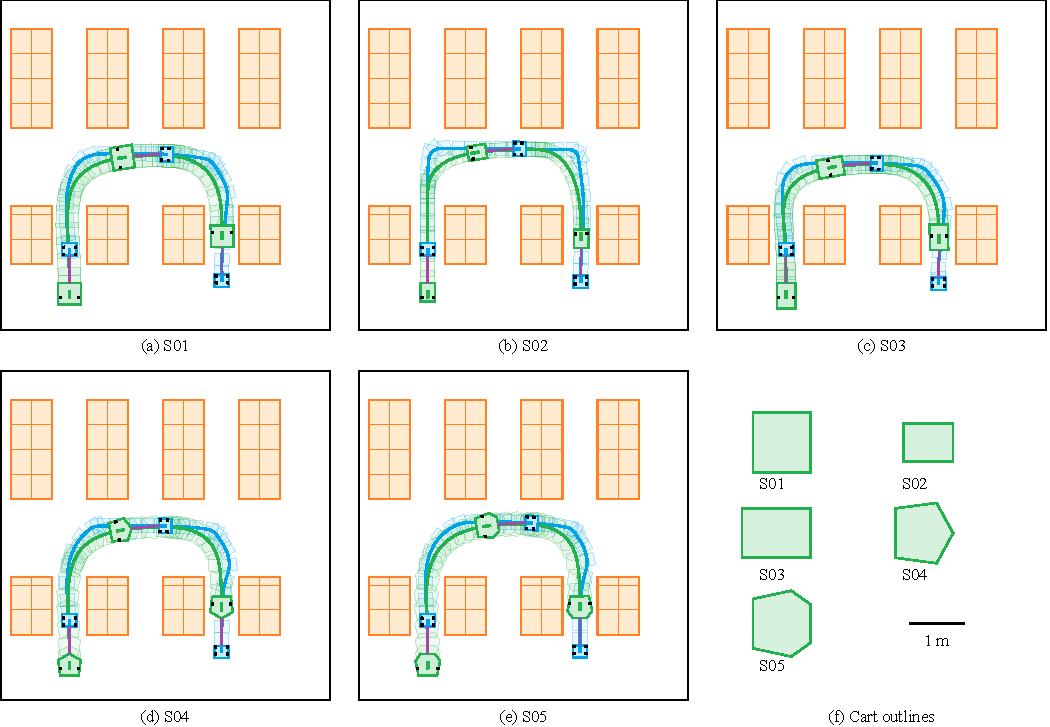
\includegraphics[width=.915\textwidth]{shape_trajectories.pdf}
\caption{Five convex cart geometries planned in the unchanged shape-test warehouse.}
\label{fig:shapes}
\end{figure*}

The serial example connects three passive carts with individual convex footprints and rear attachment points. Recursive application of~\eqref{eq:serial} produces a constructive route through another $16\times16$ m rack environment. Body separation, endpoint lengths, and nonreversing conditions are checked at every replay substep. Cable routes are checked at the original control boundaries and the corresponding boundary configurations from finer integration. This example evaluates serial kinematic feasibility. Figure~\ref{fig:train} shows the occupied route and two maneuver configurations.
The three-cart construction passes the recursive kinematic and geometric checks, with minimum body clearances of 0.178 m on the original grid and 0.204 m on finer replay. This constructive demonstration extends the prescribed per-node cable-routing model to serial towing. Physical multi-cart operation additionally requires continuous cable handling and cable--cable interaction assessment.


\begin{figure*}[!t]
\centering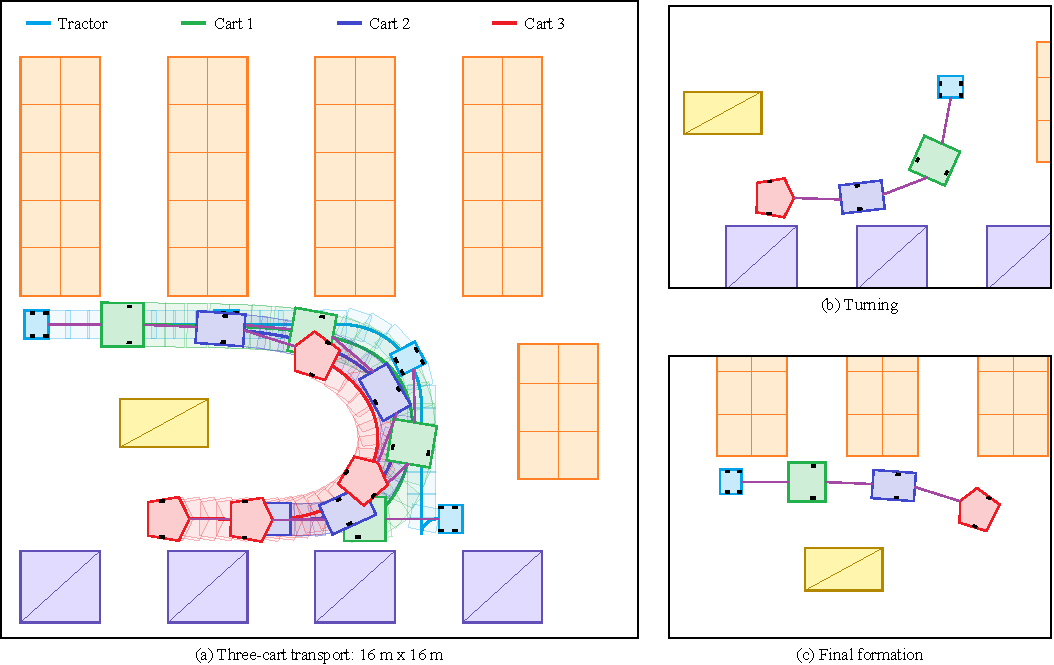
\includegraphics[width=.915\textwidth]{train_extension.pdf}
\caption{A three-cart formation navigating a confined square warehouse with individual convex footprints.}
\label{fig:train}
\end{figure*}
